% Based on: https://texample.net/tikz/examples/consort-flowchart/
%
% Create a .pdf using:
%   > pdflatex flow.tex
%
% Create a .eps using:
%   > latex  flow.tex
%   > dvips  flow.dvi
%   > ps2eps flow.ps
%
% Convert to a high-res PNG using:
% sips -s format png --resampleWidth 10000 flow.pdf --out flow.png

\documentclass{article}
\usepackage[latin1]{inputenc}
\usepackage{tikz}
\usetikzlibrary{shapes,arrows}
\usepackage{enumitem}

\newcommand*{\h}{\hspace{5pt}}% for indentation
\newcommand*{\hh}{\h\h}% double indentation

\begin{document}
\pagestyle{empty}
\pagecolor{white}
\begin{center}
  % setting the typeface to sans serif and the font size to small
  % the scope local to the environment
  \sffamily
  \footnotesize
  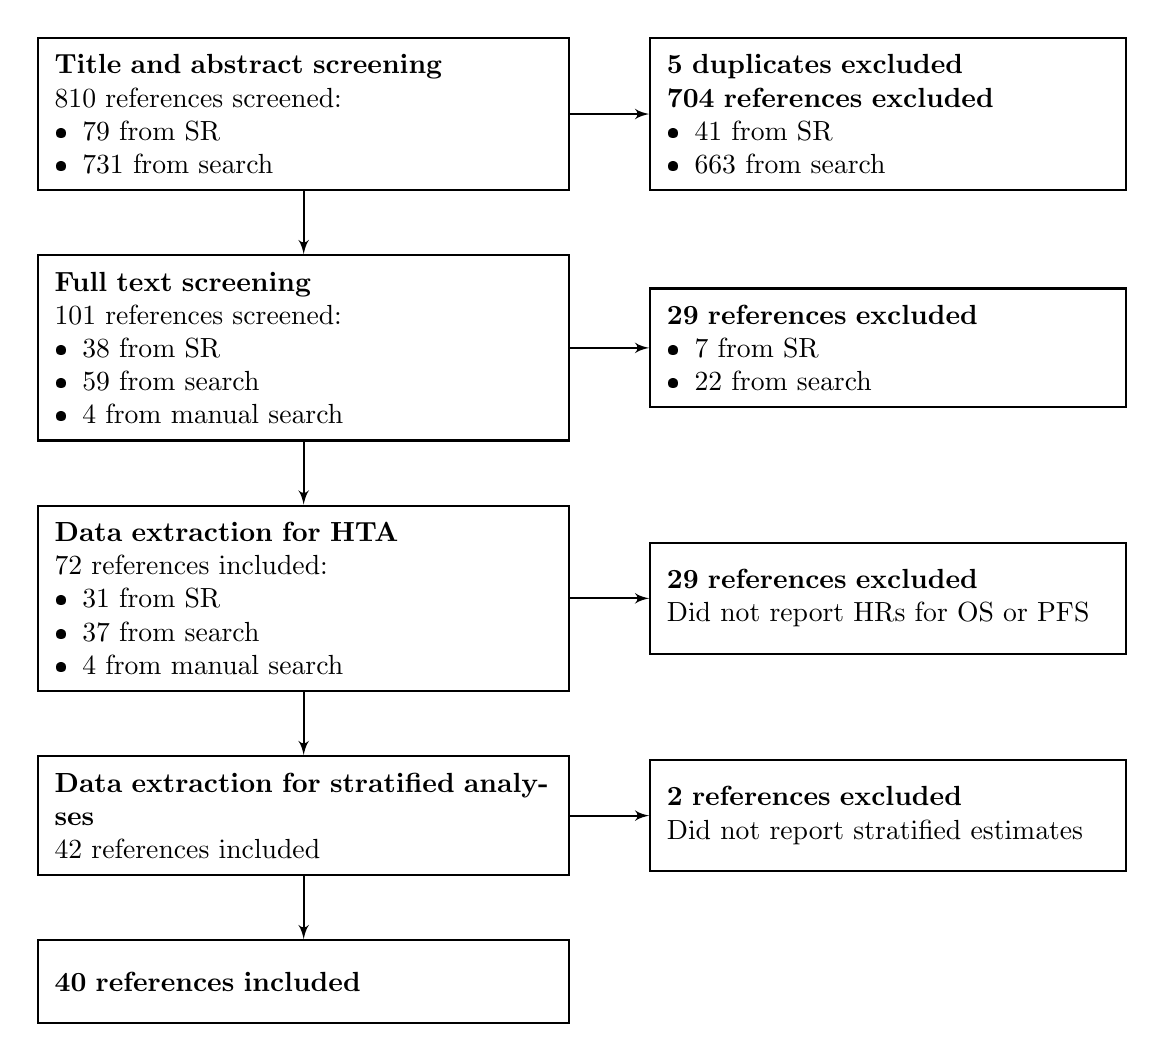
\begin{tikzpicture}[auto,
    block_center/.style ={rectangle, draw=black, thick, fill=white,
      text width=8em, text centered,
      minimum height=4em},
    block_left/.style ={rectangle, draw=black, thick, fill=white,
      text width=16em, text ragged, minimum height=4em, inner sep=6pt},
    block_noborder/.style ={rectangle, draw=none, thick, fill=none,
      text width=18em, text centered, minimum height=1em},
    block_assign/.style ={rectangle, draw=black, thick, fill=white,
      text width=18em, text ragged, minimum height=3em, inner sep=6pt},
    block_lost/.style ={rectangle, draw=black, thick, fill=white,
      text width=16em, text ragged, minimum height=3em, inner sep=6pt},
      line/.style ={draw, thick, -latex', shorten >=0pt}]
    % outlining the flowchart using the PGF/TikZ matrix function
    \matrix [column sep=10mm,row sep=8mm] {
      % Title and abstract screening
      \node [block_assign] (assessment) {\textbf{Title and abstract screening} \\
        810 references screened: \\
          \begin{itemize}[leftmargin=*, nolistsep]
            \item 79 from SR
            \item 731 from search
          \end{itemize}
      };
      & \node [block_left] (excluded1) {
        \textbf{5 duplicates excluded\\
                704 references excluded} \\
          \begin{itemize}[leftmargin=*, nolistsep]
            \item 41 from SR
            \item 663 from search
          \end{itemize}}; \\
      % Full text screening
      \node [block_assign] (full_text) {\textbf{Full text screening} \\
        101 references screened:
        \begin{itemize}[leftmargin=*, nolistsep]
          \item 38 from SR
          \item 59 from search
          \item 4 from manual search
        \end{itemize}
      };
      & \node [block_left] (excluded2) {\textbf{29 references excluded} \\
          \begin{itemize}[leftmargin=*, nolistsep]
            \item 7 from SR
            \item 22 from search
          \end{itemize}}; \\
      % Data extraction 1
      \node [block_assign] (data1) {\textbf{Data extraction for HTA} \\
        72 references included:
        \begin{itemize}[leftmargin=*, nolistsep]
          \item 31 from SR
          \item 37 from search
          \item 4 from manual search
        \end{itemize}};
      & \node [block_left] (excluded3) {\textbf{29 references excluded} \\
          Did not report HRs for OS or PFS}; \\
      % Data extraction 2
      \node [block_assign] (data2) {\textbf{Data extraction for stratified analyses} \\
        42 references included};
      & \node [block_left] (excluded4) {\textbf{2 references excluded} \\
          Did not report stratified estimates}; \\
      % Included
      \node [block_assign] (included) {\textbf{40 references included}};\\
    };% end matrix
    % connecting nodes with paths
    \begin{scope}[every path/.style=line]
      % paths for enrollemnt rows
      \path (assessment) -- (excluded1);
      \path (assessment) -- (full_text);
      \path (full_text) -- (excluded2);
      \path (full_text) -- (data1);
      \path (data1) -- (excluded3);
      \path (data1) -- (data2);
      \path (data2) -- (excluded4);
      \path (data2) -- (included);
    \end{scope}
  \end{tikzpicture}
\end{center}
\end{document}
